\documentclass[aspectratio=169,xcolor=x11names]{beamer}
\usetheme[
	titleformat=smallcaps, % Don't use pdfLatex if you want the smallcaps effect.
	titleformat subtitle=regular,
]{metropolis}

\usepackage{fontspec}
\setsansfont{Comic Sans MS}

\usepackage{array}

\title{Dynamic Binary Optimization}
\subtitle{A comprehensive comparison between Dynamo, DynamoRIO, ADORE/Itanium, and ADORE/Sparc}

\date{June 8, 2017}
\author{Chih-Yung Liang \& Shih-Kai Lin}
\institute[NTU CSIE]{Department of Computer Science and Information Engineering,\\National Taiwan University}

\begin{document}
	\maketitle
	
	\begin{frame}{Outline}
		\tableofcontents[
			hidesubsections,
		]
	\end{frame}
	
	\section{Dynamic Binary Optimization}
	\begin{frame}{Introduction}
	Dynamic Binary Optimization (DBO) aims to improve the \alert{performance} of an executing native program.
	\end{frame}

	\begin{frame}{Why Static Optimization is Insufficient?}
		\begin{description}
			\item[Analysis Scope] \hfill \\
				Cross-module optimization is complex and even unavailable, especially for dynamic linked/shared libraries.
			\item[Machine Dependent Optimization] \hfill \\
				Code optimized statically are not optimal for every micro-architecture.
			\item[Behavior Information] \hfill \\
				Behavior of some program vary greatly for different inputs. However, static optimizers can only rely on past profile data, which is not as accurate as those retrieved in runtime.
			\item[Aggressiveness] \hfill \\
				Aggressive optimizations applied speculatively by static optimizers are not revertible even they are eventually not giving good effect on the performance or causing incorrectness.
		\end{description}
	\end{frame}

	\begin{frame}{Challenges}
		\begin{itemize}
			\item The \textbf{overhead} of performing optimizations are parts of execution time.
			\item The dynamic optimizer has to realize the \textbf{hotspot} of the program.
			\item The optimizer has to be \textbf{transparent} to the target program.
		\end{itemize}
	\end{frame}

	\begin{frame}{Timeline}
		\def\arraystretch{2}
		
		\begin{tabular}{@{\,}r <{\hskip 2pt} !{\color{LightSteelBlue3}\makebox[0pt]{\textbullet}\hskip-0.5pt\vrule width 1pt\hspace{\labelsep}} >{\raggedright\arraybackslash}p{2.7cm} p{8cm}}
			\textbf{PLDI}'00 & Dynamo (\texttt{PA-8000}) & \textit{Dynamo: A Transparent Dynamic Optimization System} \\
			\textbf{CGO}'03 & DynamoRIO (\texttt{IA-32}) & \textit{An Infrastructure for Adaptive Dynamic Optimization} \\
			\textbf{JILP}'04 & ADORE (\texttt{Itanium 2}) & \textit{Design and Implementation of a Lightweight Dynamic Optimization System} \\
			\textbf{MICRO}'05 & ADORE (\texttt{UltraSPARC}) & \textit{Dynamic Helper Threaded Prefetching on the Sun UltraSPARC\textregistered\ CMP Processor} \\
		\end{tabular}
	\end{frame}
	
	\section{Optimization Mechanisms}
	\subsection{Profiling}
	\begin{frame}{Mechanisms}
		\tableofcontents[currentsection,currentsubsection]
	\end{frame}

	\begin{frame}{Startup}
		In convenience to modify the target program, it is better to have the dynamic optimizer share the \textbf{same address space} with the target program. As a result, optimizers are often built as \alert{shared libraries} and loaded into the target process using following methods:
		\begin{itemize}
			\item The target application \textbf{explicitly call} a routine starting the optimizer.
			\begin{itemize}
				\item Dynamo
			\end{itemize}
			\item Use a modified C runtime (\texttt{libc\_start\_main}) to start the optimizer.
			\begin{itemize}
				\item Dynamo
				\item ADORE
			\end{itemize}
			\item Have the program loader to preload it by setting the environment variable \texttt{LD\_PRELOAD}.
			\begin{itemize}
				\item ADORE
			\end{itemize}
		\end{itemize}
	\end{frame}
	
	\begin{frame}{Interpretation}
		The optimizer has to realize the hotspot of the executing program, which is usually viewed as code that are \textbf{executed many times}.
		
		\alert{Dynamo} starts to run a program using a lightweight \alert{software interpreter} to count execution frequencies of code sequences.
		
		Frequently executed code sequences are selected as \alert{traces} to optimize. Generated native versions of traces (called \alert{fragment}) are stored in the \alert{code cache}. After that, future executions of these traces use the native code in the code cache instead of interpreting.
	\end{frame}

	\begin{frame}{Trace}
		Dynamo defines \textit{start-of-trace} as \textbf{targets of backward-taken branches}, which are likely loop headers, and fragment cache exit branches. \textit{End-of-trace} are \textbf{backward-taken branches} or taken branches whose targets correspond to the entry point.
		
		A fragment is built as an optimized \textbf{single-entry, multi-exit} contiguous sequence of instructions.
	\end{frame}

	\begin{frame}{Cached Interpretation}
		To overcome the high overhead caused by the interpretation, \alert{DynamoRIO} \textbf{caches} translations of frequently executed code. It copies \textbf{basic blocks} into code cache and executes them natively. At the end of a block, the machine state is saved and control is returned to DynamoRIO. The interpretation overhead is furthermore decreased with following additional optimizations:
		
		\begin{center}
			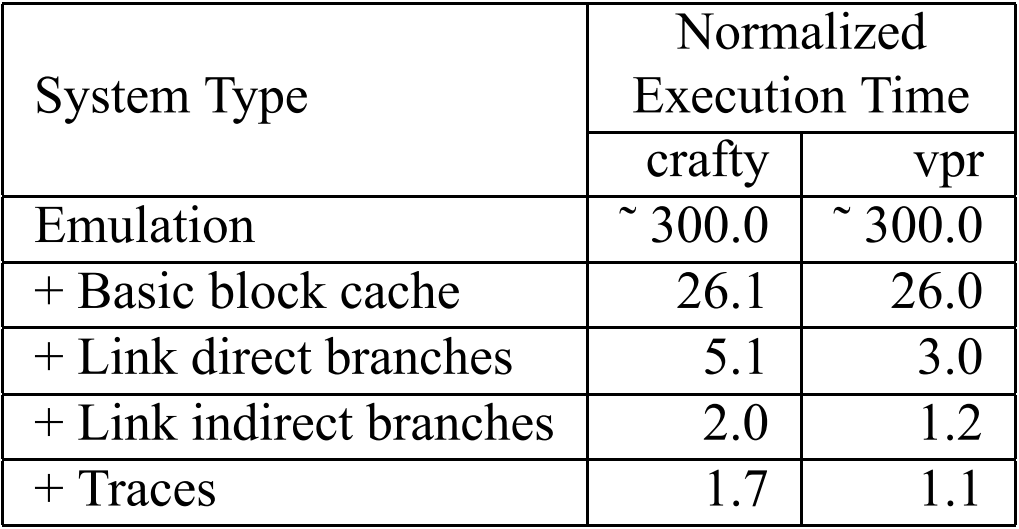
\includegraphics[width=0.5\textwidth]{DynamoRIO-interpretation-cache}
		\end{center}
	\end{frame}

	\begin{frame}{Sampling-based Profiling}
		\alert{ADORE} utilizes \textit{Itanium 2}'s \textbf{Performance Monitoring Unit} (PMU) and some system services to figure out the hotspot of an executing program, so the target program is \textbf{run natively}. The trace building and optimizing are done in \textbf{the other thread}, which is run on the other physical core.
		
		\begin{center}
			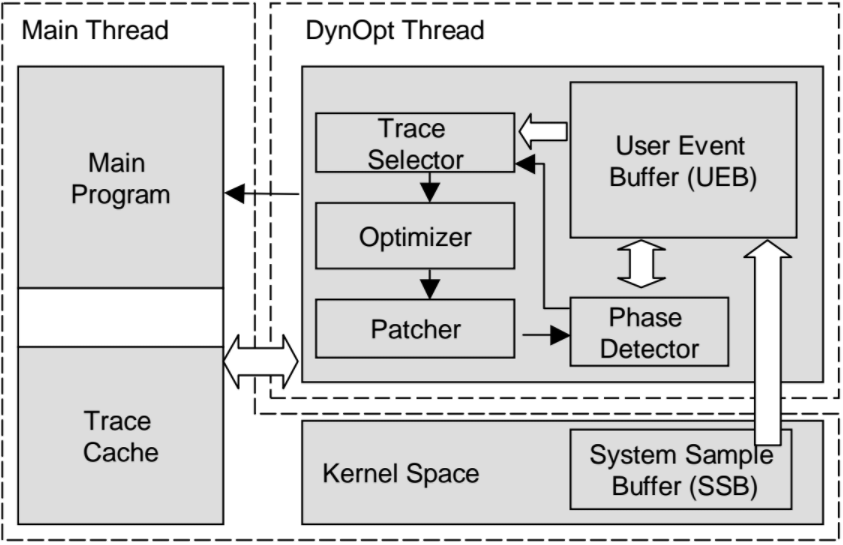
\includegraphics[width=0.5\textwidth]{ADORE-framework}
		\end{center}
	\end{frame}

	\begin{frame}{Phase Detection}
		Programs have phases. It is more meaningful to optimize code in \textbf{stable phase}.
		\begin{block}{}
			\begin{columns}
				\begin{column}[T]{0.46\linewidth}
					\alert{Dynamo} \textbf{flushes} its code cache when the fragment creation rate has a sharp increase.
					\begin{center}
						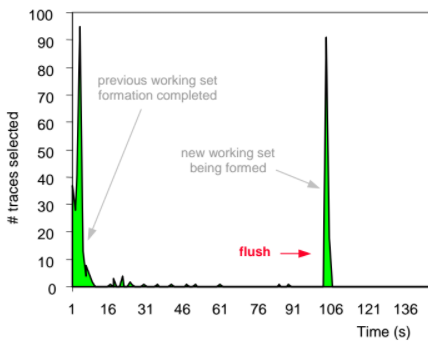
\includegraphics[width=0.8\textwidth]{Dynamo-flush}
					\end{center}
				\end{column}
				\begin{column}[T]{0.46\linewidth}
					\alert{ADORE} monitors \textbf{PC} and \textbf{CPI} for phase stability and performs optimizations only when stable.
					\begin{center}
						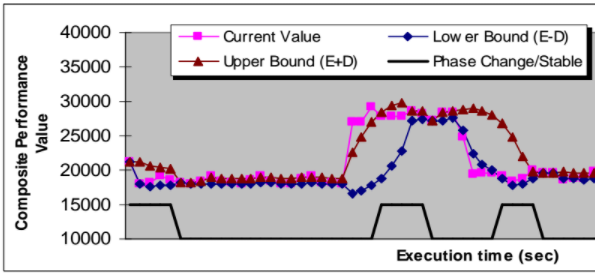
\includegraphics[width=\textwidth]{ADORE-phase}
					\end{center}
				\end{column}
			\end{columns}
		\end{block}
	\end{frame}
	
	\subsection{Optimizations}
	\begin{frame}{Mechanisms}
		\tableofcontents[currentsection,currentsubsection]
	\end{frame}

	\begin{frame}{Optimizations in Dynamo}
		\begin{columns}
			\begin{column}[T]{0.5\linewidth}
				\begin{block}{Conservative Optimizations}
					\begin{itemize}
						\item Redundant branch elimination
						\item Redundant assignment elimination
						\item Copy/constant propagation
						\item Strength reduction
						\item Loop unrolling
					\end{itemize}
				\end{block}
			\end{column}
			\begin{column}[T]{0.5\linewidth}
				\begin{block}{Aggressive Optimizations}
					\begin{itemize}
						\item Dead code removal
						\item Code sinking
						\item Loop invariant code motion
						\item Redundant load removal %it relies on symbol table for information about volatile variable
					\end{itemize}
				\end{block}
			\end{column}
		\end{columns}
		
		Since Dynamo is interpretation-based and use little hardware support, it is hard to realize and optimize various types of performance behavior, such as \textbf{cache} and \textbf{branch prediction}.
	\end{frame}

	\begin{frame}{Optimization Examples in DynamoRIO}
		DynamoRIO is a \textbf{framework} for implementing dynamic analysis and optimizations. The paper describes several example DynamoRIO clients.
		\begin{itemize}
			\item Redundant load removal %It still wins static optimizers because it can cross basic block boundary.
			\item Strength reduction %inc -> add 1
			\item Indirect branch dispatch %Predict one common target
			\item Custom traces %to inline entire procedure call into a trace. That is, to make the `call` the start-of-trace, and make the `return` the end-of-trace
		\end{itemize}
	\end{frame}

	\begin{frame}{Optimization in ADORE/Itanium (Prediction-based Prefetch)}
		ADORE focuses on inserting \textbf{cache prefetches} into fragments to decrease the amount of cache misses. % cache miss and branch prediction are hard to optimize statically.
		
		\begin{columns}
			\begin{column}[T]{0.42\linewidth}
				\begin{block}{Steps}
					\begin{enumerate}
						\item Tracking \alert{delinquent loads} %cache miss latency more than 8 cycles implies an L2 or L3 miss.
						\item Data reference pattern detection
						\item Prefetch generation % no inst like fetch[r11+80]. Has to calculate actual address. Distance
						\item Prefetch code optimization and scheduling % for redundancy. In addition, IA64 is VLIW, so requiring scheduling to preventing wasting empty slots and increase number of bundles.
					\end{enumerate}
				\end{block}
			\end{column}
			\begin{column}[T]{0.58\linewidth}
				\begin{exampleblock}{Data Reference Pattern}
					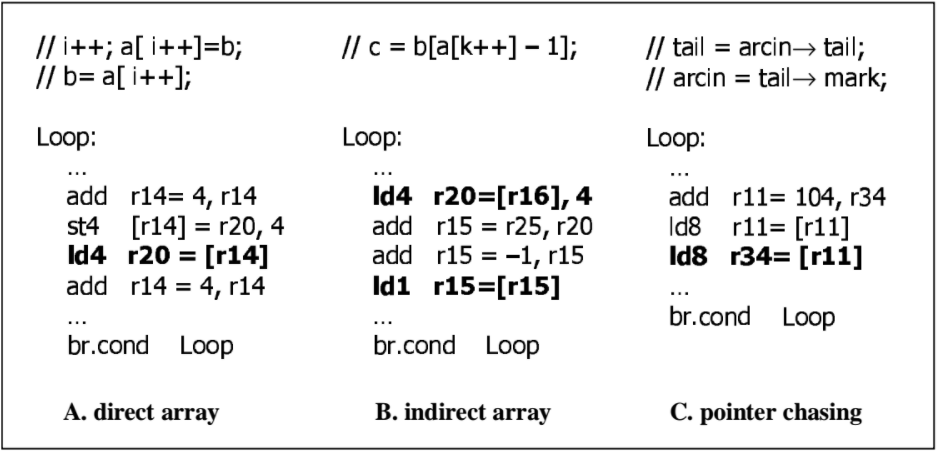
\includegraphics[width=\textwidth]{ADORE-pattern}
				\end{exampleblock}
			\end{column}
		\end{columns}
	\end{frame}

	\begin{frame}{Optimization in ADORE/SPARC (Execution-based Prefetch)}
		\alert{Execution-based profiling} can provide better prefetching \textit{coverage} and \textit{accuracy}. It is especially suitable for the dual-core UltraSPARC, which has \textbf{private L1 caches} for each core and a \textbf{shared L2 cache}.
		
		Extended from ADORE/Itanium, it makes the optimization thread also a \alert{helper thread}, which executes a \textbf{distilled version} (called \alert{scouting code}) of the forward slice starting from the missing load. The distillation includes:
		\begin{itemize}
			\item Memory stores and unrelated instructions are ignored, leaving only delinquent loads and instructions changing the control flow.
			\item Delinquent loads are replaced by \textbf{strong prefetches} unless their results are used by subsequent computations.
			\item Otherwise, delinquent loads are converted into \textbf{non-faulting loads}.
		\end{itemize}
	\end{frame}

	\subsection{Performance}
	\begin{frame}{Mechanisms}
		\tableofcontents[currentsection,currentsubsection]
	\end{frame}

	\begin{frame}{Performance - Dynamo}
		\begin{columns}
			\begin{column}[b]{0.5\linewidth}
				\begin{itemize}
					\item Average speedup: 9\%
					\begin{itemize}
						\item Mainly from trace selection
					\end{itemize}
					\item Long execution time
					\begin{itemize}
						\item \alert{ijpeg} performs badly
					\end{itemize}
				\end{itemize}
			\end{column}
			\begin{column}[b]{0.5\linewidth}
				\begin{itemize}
					\item Stable working set
					\begin{itemize}
						\item \alert{li}, \alert{m99skim}, \alert{perl}, and \alert{compress}
						\item \alert{go} and \alert{vortex} on the contrary
					\end{itemize}
				\end{itemize}
			\end{column}
		\end{columns}
		\begin{center}
			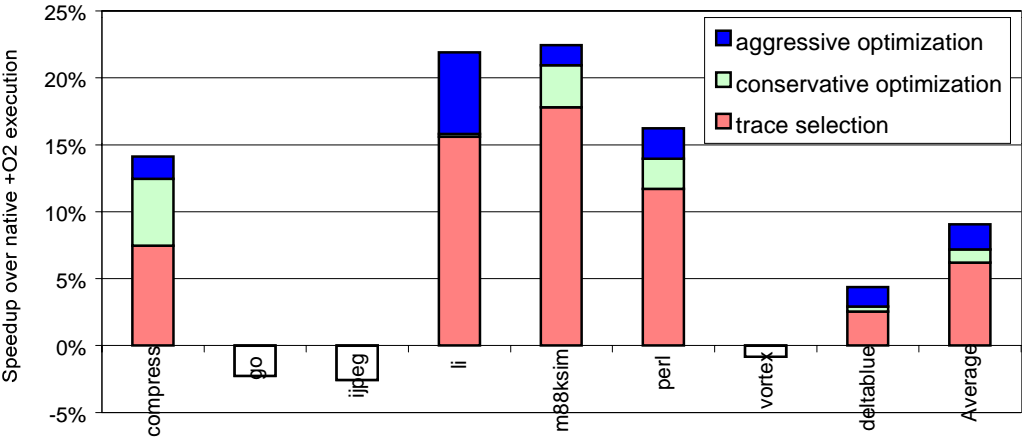
\includegraphics[width=0.7\textwidth]{Dynamo-speedup}
		\end{center}
	\end{frame}

	\begin{frame}{Performance - Dynamo}
		\begin{itemize}
			\item Specific to the architecture (code generated by the compiler, implementation)
			\begin{itemize}
				\item Branch misprediction penalty is 5 cycles.
				\item Indirect Branch are always mispredicted.
			\end{itemize}
			\item Large instruction cache
			\begin{itemize}
				\item Gain from I-cache locality improvement is not significant.
			\end{itemize}
			\item Unified instruction and data TLB with only 96 entries
			\begin{itemize}
				\item Better locality of the working set in the fragment cache results in better performance.
			\end{itemize}
		\end{itemize}
	\end{frame}

	\begin{frame}{Performance - DynamoRIO}
		\begin{columns}
			\begin{column}{0.45\linewidth}
				\begin{itemize}
					\item FP benchmark: 12\% speedup on average
					\begin{itemize}
						\item Redundant load removal (\texttt{rlr})
						\begin{itemize}
							\item Static compilation is limited by basic block.
						\end{itemize}
						\item Strength reduction
						\begin{itemize}
							\item Optimized for specific architecture
							\item \texttt{inc} is slower than \texttt{add 1} on \textit{Pentium 4} but faster on \textit{Pentium 3}
						\end{itemize}
						\item Indirect branch dispatch
						\begin{itemize}
							\item Inline indirect branch targets when building the trace
						\end{itemize}
					\end{itemize}
				\end{itemize}
			\end{column}
			\begin{column}{0.55\linewidth}
				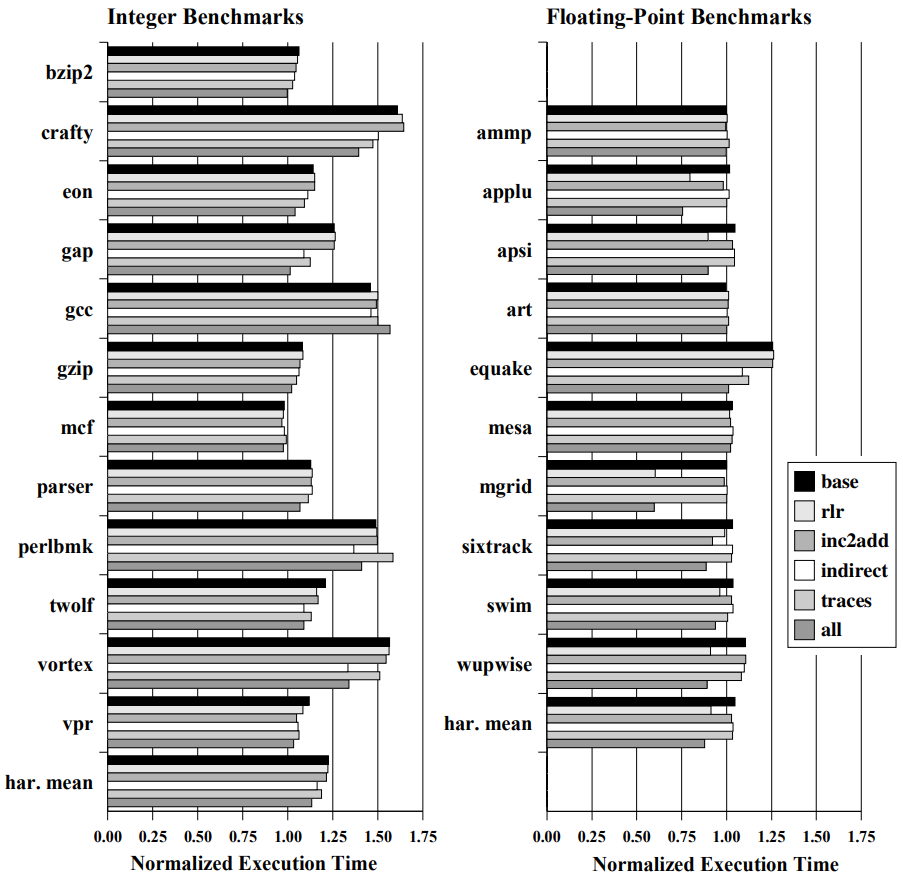
\includegraphics[width=\textwidth]{DynamoRIO-speedup}
			\end{column}
		\end{columns}
	\end{frame}

	\begin{frame}{Performance - DynamoRIO}
		The overhead comes from:
		\begin{itemize}
			\item Indirect branches handling
			\begin{itemize}
				\item Indirect branches (including \textbf{returns} and \textbf{indirect calls}) are translated into indirect jumps.
				\item The hardware has return address predictors but no indirect jump predictors.
				\item Misprediction cost is higher than native.
			\end{itemize}
			\item Dealing with \texttt{eflags} changes caused by introduced code.
		\end{itemize}
	\end{frame}

	\begin{frame}{Performance - ADORE}
		Cache misses on Itanium machines have significant impact on performance.
		
		\begin{columns}
			\begin{column}{0.4\linewidth}
				\begin{itemize}
					\item \texttt{O2} + reserve registers
					\begin{itemize}
						\item Without static prefetch
						\item Speedup: 3\%--57\%
						\item No effect: -2\%--1\%
					\end{itemize}
					\item \texttt{O3} + reserve registers
					\begin{itemize}
						\item With \textbf{static prefetch}
						\item Speedup: 11\%--22\%
						\item No effect: -3\%--2\%
					\end{itemize}
				\end{itemize}
			\end{column}
			\begin{column}{0.6\linewidth}
				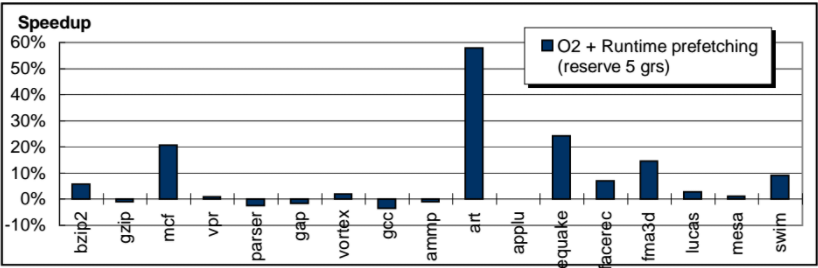
\includegraphics[width=\textwidth]{ADORE-speedup1}\\
				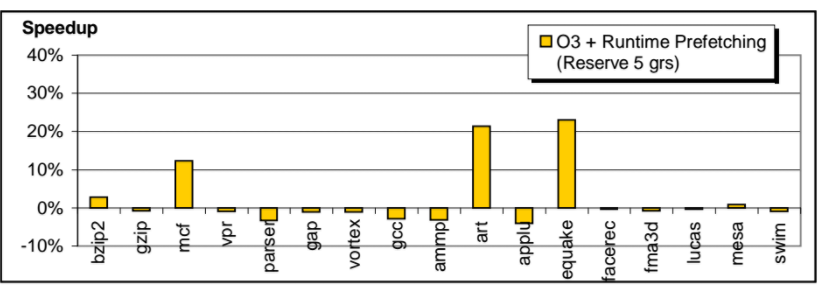
\includegraphics[width=\textwidth]{ADORE-speedup2}
			\end{column}
		\end{columns}
	\end{frame}

	\begin{frame}{Performance - ADORE}
		\begin{itemize}
			\item Overhead is trivial (average: 2\%).
			\begin{itemize}
				\item Contiguous sampling, phase detection, trace optimization
			\end{itemize}
		\end{itemize}
	
		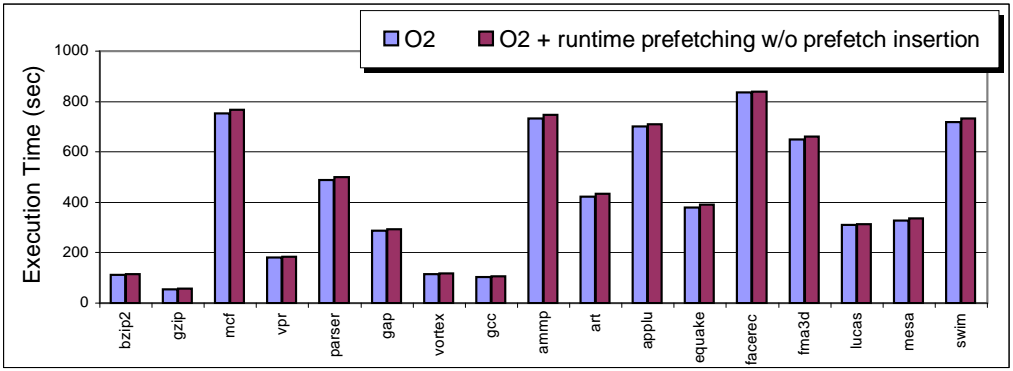
\includegraphics[width=\textwidth]{ADORE-overhead}
	\end{frame}

	\begin{frame}{Performance - Helper-threaded prefetch}
		\begin{itemize}
			\item Max speedup: 35\% (\alert{mcf})
			\begin{itemize}
				\item Memory Level Parallelism (MLP) helps hide latency by overlapping cache misses.
			\end{itemize}
			\item Overhead: 1\%--2\%
		\end{itemize}
		\begin{columns}
			\begin{column}[T]{0.4\linewidth}
				\begin{alertblock}{Fluent}
					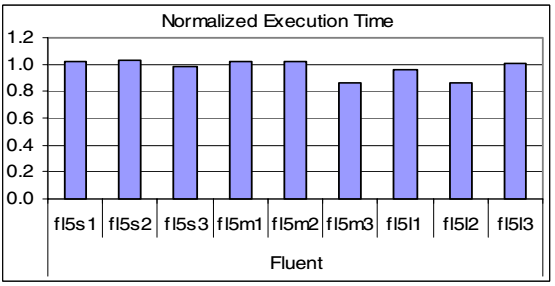
\includegraphics[width=\textwidth]{ADORE2-fluent}
				\end{alertblock}
			\end{column}
			\begin{column}[T]{0.6\linewidth}
				\begin{alertblock}{SPEC2000}
					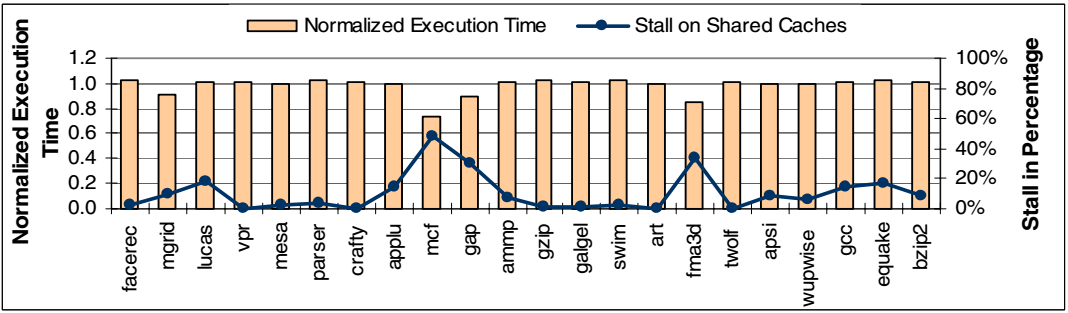
\includegraphics[width=\textwidth]{ADORE2-SPEC-base}\\
					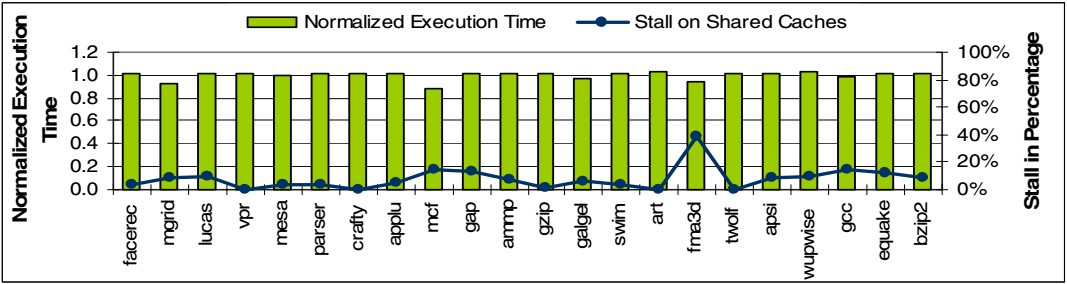
\includegraphics[width=\textwidth]{ADORE2-SPEC-peak}
				\end{alertblock}
			\end{column}
		\end{columns}
	\end{frame}

	\begin{frame}{Performance - Helper-threaded prefetch}
		\begin{itemize}
			\item Particularly effective on hiding L3 cache miss latency.
			\item Does not decrease L1 data cache miss penalty (\texttt{L2\_Hit\_Stall}).
		\end{itemize}
		
		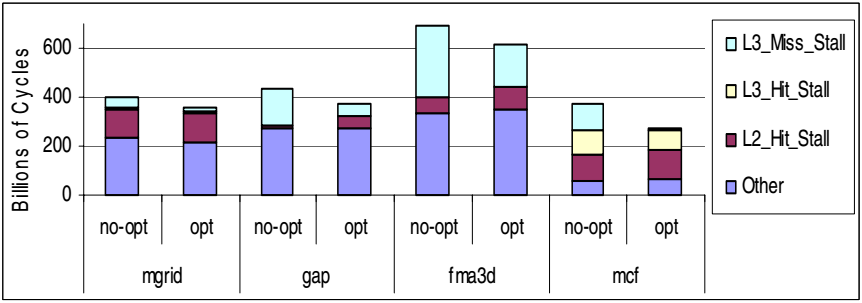
\includegraphics[width=\textwidth]{ADORE2-cycle}
	\end{frame}
	
	\section{Comparison}
	\begin{frame}{Comparison}
		\scriptsize
		\begin{tabular}{p{2.6cm}||p{2.5cm}|p{2.5cm}|p{2.2cm}|p{2.2cm}}
			& Dynamo & DynamoRIO & ADORE/Itanium & ADORE/SPARC \\
			\hline
			\hline
			Profile (Overhead) & \multicolumn{2}{p{5cm}|}{\centering Interpretation (High)} & \multicolumn{2}{p{4.4cm}}{\centering Sampling-based profiling (Low)} \\
			\hline
			Target\newline architecture & HP PA-RISC & IA-32 & Itanium 2 & UltraSPARC\newline (Panther) \\
			\hline
			Optimization & \multicolumn{2}{p{5cm}|}{Redundant load/branch/assignment elimination, copy/constant propagation, strength reduction, LICM, and unrolling} & Prediction-based prefetch & Execution-based profiling \\
			\hline
			Speedup & Avg: 9\%\newline Max: 22\% & Floating avg: 12\%\newline Max: 40\% & 3--57\% & Max: 35\% \\
			\hline
			Mainly gain from & Code layout and\newline indirect branch &  & \multicolumn{2}{p{4.4cm}}{\centering Decreased cache miss penalty} \\
			\hline
			Performance impact when no gain & High (Bailout) & High (Mean 12\%) & Low (Avg: 2\%) & Low (1--2\%)\\
		\end{tabular}
	\end{frame}
	
	\section{Conclusion}
	\begin{frame}{Conclusion}
		\begin{itemize}
			\item Dynamic optimization can deal with some problems that cannot be done statically.
			\begin{itemize}
				\item Cache misses \& branch misprediction patterns are difficult to optimize at static time.
				\item Find the hot code and optimize.
			\end{itemize}
			\item Sampling-based profiling has negligible overhead.
			\begin{itemize}
				\item But need more time to collect enough data.
			\end{itemize}
			\item Static + Dynamic integration?
			\begin{itemize}
				\item Annotation on may-be-hot code.
			\end{itemize}
			\item Multi-threaded programs are increasing.
			\begin{itemize}
				\item ADORE/COBRA can optimize for multi-cores.
			\end{itemize}
		\end{itemize}
	\end{frame}

	\begin{frame}[standout]
		Q \& A
	\end{frame}

	\appendix
	\begin{frame}[fragile]{Current DynamoRIO}
		DynamoRIO announced 7.0 release candidate (4 Feb, 2017) which contains \alert{support for AArch64}. Until now, DynamoRIO supports:
		
		\begin{columns}
			\begin{column}[T]{0.4\linewidth}
				\begin{block}{Architectures:}
					\begin{enumerate}
						\item IA-32
						\item AMD64
						\item ARM
						\item AArch64
					\end{enumerate}
				\end{block}
			\end{column}
			\begin{column}[T]{0.4\linewidth}
				\begin{block}{Operating Systems:}
					\begin{enumerate}
						\item Windows
						\item Linux
						\item Android
					\end{enumerate}
				\end{block}
			\end{column}
		\end{columns}
	
		It is now a open source project with binary packages available: {\color{blue}https://github.com/DynamoRIO/dynamorio}
		
		There will be a tutorial on DynamoRIO held at \textbf{CGO 2017}.
	\end{frame}
\end{document}